\documentclass[10pt,twocolumn,letterpaper]{article}

\usepackage{statcourse}
\usepackage{times}
\usepackage{mathtools}
\usepackage{epsfig}
\usepackage{float}
\usepackage{graphicx}
\usepackage{amsmath}
\usepackage{amssymb}
\usepackage[breaklinks=true,bookmarks=false]{hyperref}


\statcoursefinalcopy


\setcounter{page}{1}
\begin{document}

\title{Electricity Demand Forecasting (EDF) using an LSTM-based RNN}

\author{Apolline Foucher\\
{\tt\small a.foucher@mpp.hertie-school.org}
\and
Augustine Malija\\
{\tt\small a.malija@mpp.hertie-school.org}
\and
Vlad Surdea-Hernea\\
{\tt\small v.surdea-hernea@mpp.hertie-school.org}
}

\maketitle
%\thispagestyle{empty}


% MAIN ARTICLE GOES BELOW
%%%%%%%%%%%%%%%%%%%%%%%%%%%%%%%%%%%%%%%%%%%%%%%%%%%%%%%%%%%%%%%

%%%%%%%%% ABSTRACT
\begin{abstract}
   The following project \footnote{GitHub account \url{https://github.com/vladsurdea/ML}} predicts the hourly electricity demand in a given market by using a LSTM-based RNN architecture. The prediction is based on historical data of the hourly electricity load available between 2006 and 2019, in the absence of covariates describing weather events during this period. The results of the model are compared with the baseline ARIMA model, traditionally used in the transport and distribution industry to forecast demand in the day-ahead and spot markets. The ARIMA model is a standard, econometric model that does not employ ML algorithms. A combination of human and automatic evaluations is performed. The preliminary results show that the LSTM-based RNN outperforms the traditional model in multiple areas, especially when it comes to predict sudden spikes in electricity load consumption.
\end{abstract}



\section{Proposed Method}

\subsection{Theoretical approach}

To predict the hourly consumption of electricity based on historical load data in the absence of weather information, we use a LSTM-based RNN. This architecture was introduced by Hochreiter and Schmidhuber in 1997, and has been applied in recent years to the challenge of EDF. In the following lines, we offer a mathematical, brief introduction to the mechanics behind the LSTM-based RNN, that follows Muzaffar and Afshari (2019). A complete methodology will be formulated for the final version of the project.

In standard RNN architectures, the neural network is designed as a chain of identical modules formed as a series of hidden networks, usually in the form of a single sigmoid layer. In contrast to this standard architecture, the hidden layers of a LSTM-based RNN have a more complex structure capable of learning long-term dependencies. The LSTM-extension introduces the concepts of gate and memory cell in each hidden layer in the network. As a consequence, a memory block in the LSTM-based RNN is composed of four structural parts: an input gate , a forget gate , an output gate , and the self-connected memory cells:
\begin{itemize}
    \item The input gate manages the entry of the activations to the memory cells of the neural network.
    \item The output gate is designed to learn what cell activations to filter and, therefore, send as output to the successive network.
    \item The forget gate assists the neutral network to disregarding the past input data and reset the memory cells for the new inputs.
\end{itemize}
In addition to this tripartite structure, LSTM applies multiplicative gates to make it possible for the memory cells to access and store the information over a long time interval.

Briefly stated, based on the input time-series vector \textbf{x}=$\{x_1,x_2,x_3,...x_t\}$, the LSTM-based RNN will predict sequences: the hidden state sequence  \textbf{y}=$\{y_1,y_2,y_3,...y_t\}$ and the output sequence \textbf{h}=$\{h_1,h_2,h_3,...h_t\}$.The process is iterative, and is realised by sequentially updating the states of the memory cells.

The first step in the process is for the forget gate to be applied in order to decide what part of the information to discard from the cell state.The activation of the forget gate is computed via the use of a sigmoid function:

$$f_t=\sigma(W_{ix}x_t+ W_{fw}h_{t-1}+W_{fc}C_{t-1}+b_f) $$

 $f_t$ has values between 0 and 1, where 0 would mean discarding all the information from the last cell state, and 1 retaining all the information in the last cell state. Nevertheless, usually the value does not attain this extreme values.
 
After deciding what information to forget, the LSTM model decides what new information to store in the new cell state. Once again, a sigmoid function is used to determine the input gate layer. This second step is the reverse, symmetrical operation to the first step.

$$i_t=\sigma(W_{ix}x_t+W_{ih}h_{t-1}+W_{ic}C_{t-1}+b_i)$$

Potential values of the new cell states are included in a new vector, $U_t$, that is computed by using the standard sigmoid layer present in the RNN.

$$U_t=g(W_{cx}x_t+W_{ch}h_{t-1}+W_{ic}C_{t-1}+b_i) $$

The old cell state $C_{t−1}$ is updated to a new cell state $C_t$, with the support of the previously-estimated $f_t$ and $U_t$. $f_t$ is being used in order to deduce what  information to forget from the last state $C_{t−1}$ , while $U_t$ is used to understand how much new information to retain:

$$C_t=U_ti_t+C_{t-1}f_t $$

Based on this, the output gate is produced using a different sigmoid layer of the network:

$$o_t=\sigma(W_{ox}x_t+W_{oh}h_{t-1}+W_{oc}C_{t-1}+b_o$$

A cell output sigmoid activation function $\ell$ is applied over the cell state, which is then multiplied by the output $o_t$ to generate the desired information about $h_t$:

$$h_t=o_t \ell(C_t) $$

An output activation function $k$is used to produce information about the output of the memory block:

$$y_t=k(W_{yh}h_t+b_y)$$

This model will be compared to a standard, econometric ARIMA model. Currently we explore the possibility of also introducing a random forest. The specifics of both the ARIMA and potentially of the RF will be presented in the final draft.

\subsection{Coding strategy}

Our data cleaning strategy is original, while the design of the ARIMA and LSTM models follows existing sources on the internet, such as projects existing on Github \href{https://github.com/drwiiche/electricity-consumption}{already}

To implement the LSTM-based RNN architecture, we make use of a sequential model imported from Keras. We incrementally add a series of LSTM layers, choosing the appropriate dropout regularization to the sequential regressor. In this way, we mitigate the chances of over-fitting and potentially improve the performance of our model. We have experimented with different choices for the number of LSTM layers, but we observed that the improvements after the fifth are too small to notice. 

When compiling the LSTM-based RNN, we have used both the "adam" and the "rmsprop" optimizers.

The last step was to actually fit the model by using inputs from the training set. For this, we tested a a large number of combinations for both batches (the number of training samples to work through before the model’s internal parameters are updated) and epochs (the number of complete passes through the training dataset.), but ultimately chose to stick with 100 epochs and 32 batches. This will be further discussed and ultimately, we intend to compare the results of the model based on these choices.

\section{Experiments}
\paragraph{Data:} For the scope of this project, we use the historical electricity consumption database provided by the European Network of Transmission System Operators (ENTSO-E). This database encompasses a range of data-sets provided by national Transmission System Operators (ENTSO-E) in Europe. 

In this sense, we decided to focus on a sample of very different countries, in order to see whether our proposed model would generate accurate results in a variety of conditions.The countries chosen at this stage are Romania, Austria and Poland. The TSOs from these three countries have made available hourly electricity consumption data from 2006 up to 2019. For the purpose of the mid-term report, we only report the results for Romania, as this was the country on which the initial experiments have been run. The dataset provided by the Romanian TSO contains 119771 observations, one for each hour between 01.01.2006 and 31.08.2019.

The original dataset comes in the form of an xlsx file, with the data being structured in the wide format. The process of data wrangling, focused especially on changing the structure of the dataset to long has been conducted in parallel in R and Python. Additionally, we pre-processed the data in order to use the date-time (constructed from the rest of the variables) as the index of the dataset. Lastly, to include weekly and daily seasonality, we also created new variables that capture these effects: Day and Week.

The new aspect of the dataset can be observed in the figure below: 

\begin{figure}[H]
\begin{center}
   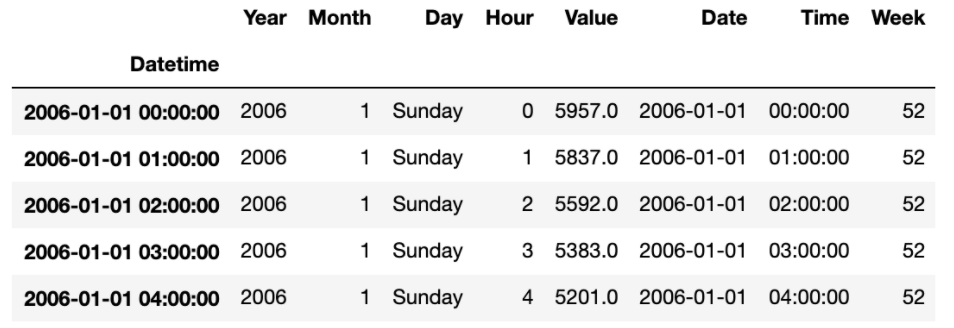
\includegraphics[width=\linewidth]{midterm-report-latex/Data2.png}
\end{center}
   \caption{Post-cleaning dataset structure}
\end{figure}
To better understand the seasonal variations and other patterns in the electricity consumption data, we analyse Figure 2 and Figure 3. Figure 2 displays the average level of electricity consumption according to the monthly distribution. In this sense, we confirm the expected spike during winter. Figure 3 plots the electricity consumption according to the hourly distribution. Once again, the expectations are confirmed: there is a significant day-night discrepancy, with more electricity being consumed on average during the 8:00-20:00 interval, with a spike in the latter part of the evenings.

\begin{figure}[H]
\begin{center}
   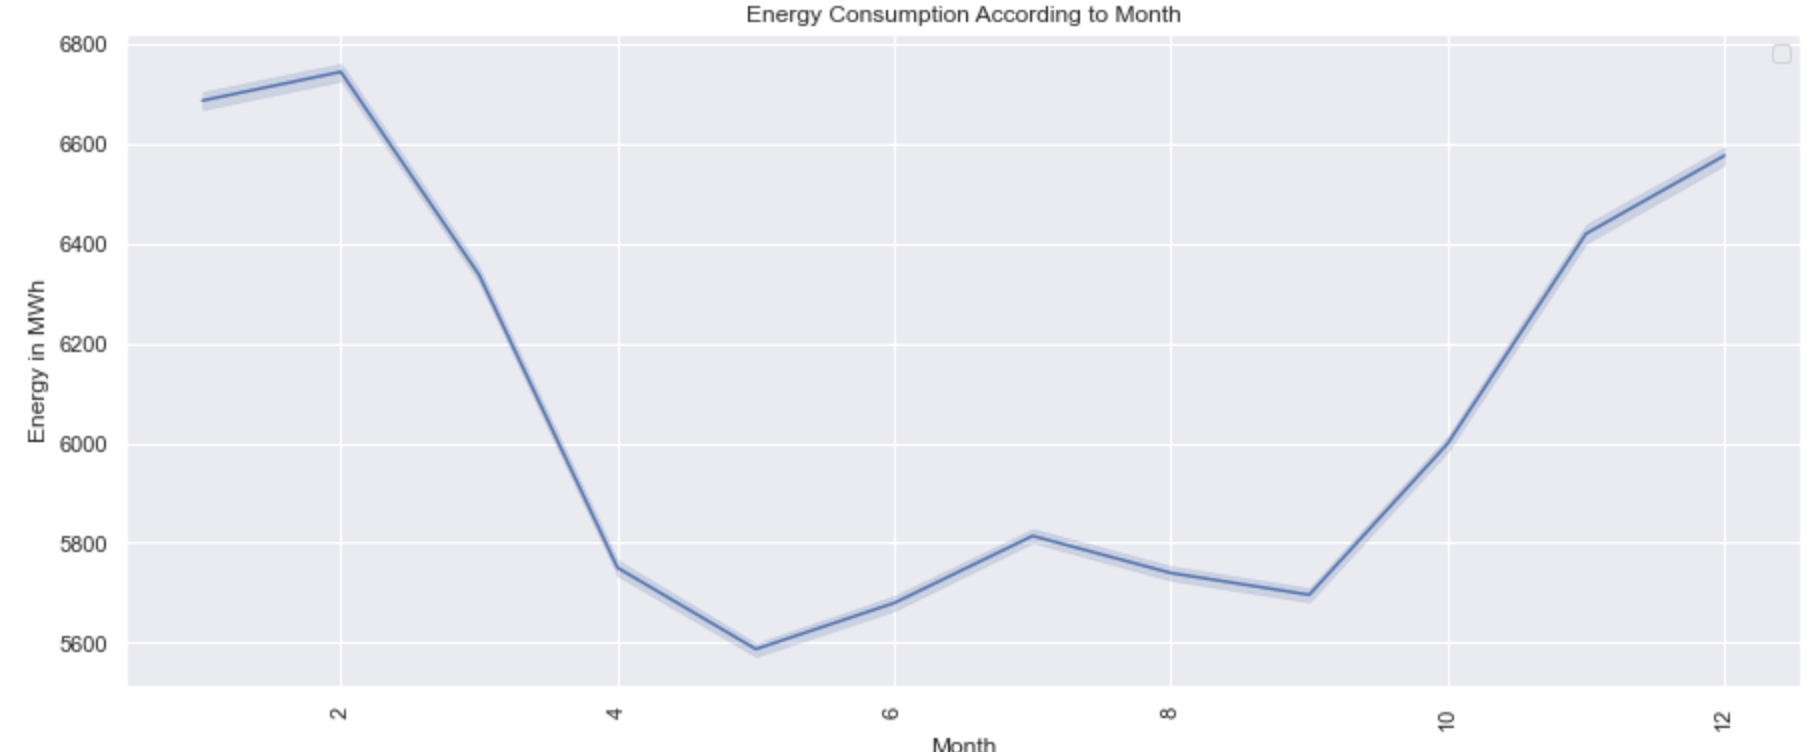
\includegraphics[width=\linewidth]{midterm-report-latex/month.png}
\end{center}
   \caption{Monthly pattern of electricity consumption}
\end{figure}

\begin{figure}[h]
\begin{center}
   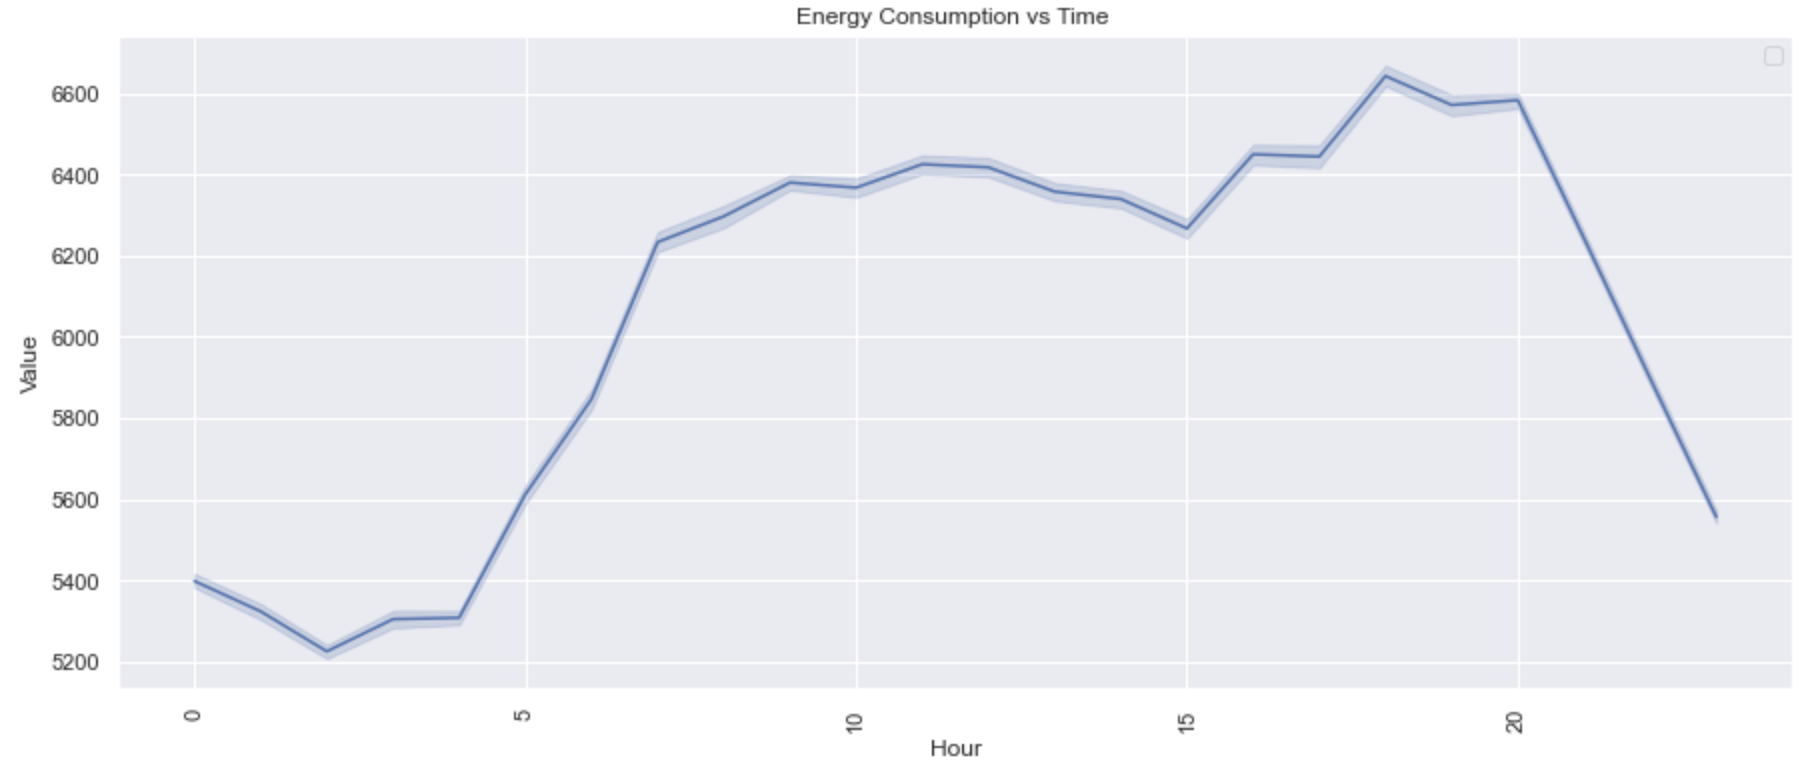
\includegraphics[width=\linewidth]{midterm-report-latex/Time.png}
\end{center}
   \caption{Hourly pattern of electricity consumption}
\label{fig:google-scholar-1col}
\end{figure}

Secondly, we analyse the overall patterns existing in electricity consumption through the histogram above. Figure 4 lets us observe, therefore, that electricity consumption follows with an almost-normal distribution centred around the 6000 MWh value. However, there are very few extreme loads, which means it will be a complicated challenge to capture these using only the historical data with the LSTM. Nevertheless, this statical point provides us with the first baseline model with which to compare the LSTM: a simple-model that would predict the average load of the previous years for each hour in the test interval. 

\begin{figure}[H]
\begin{center}
   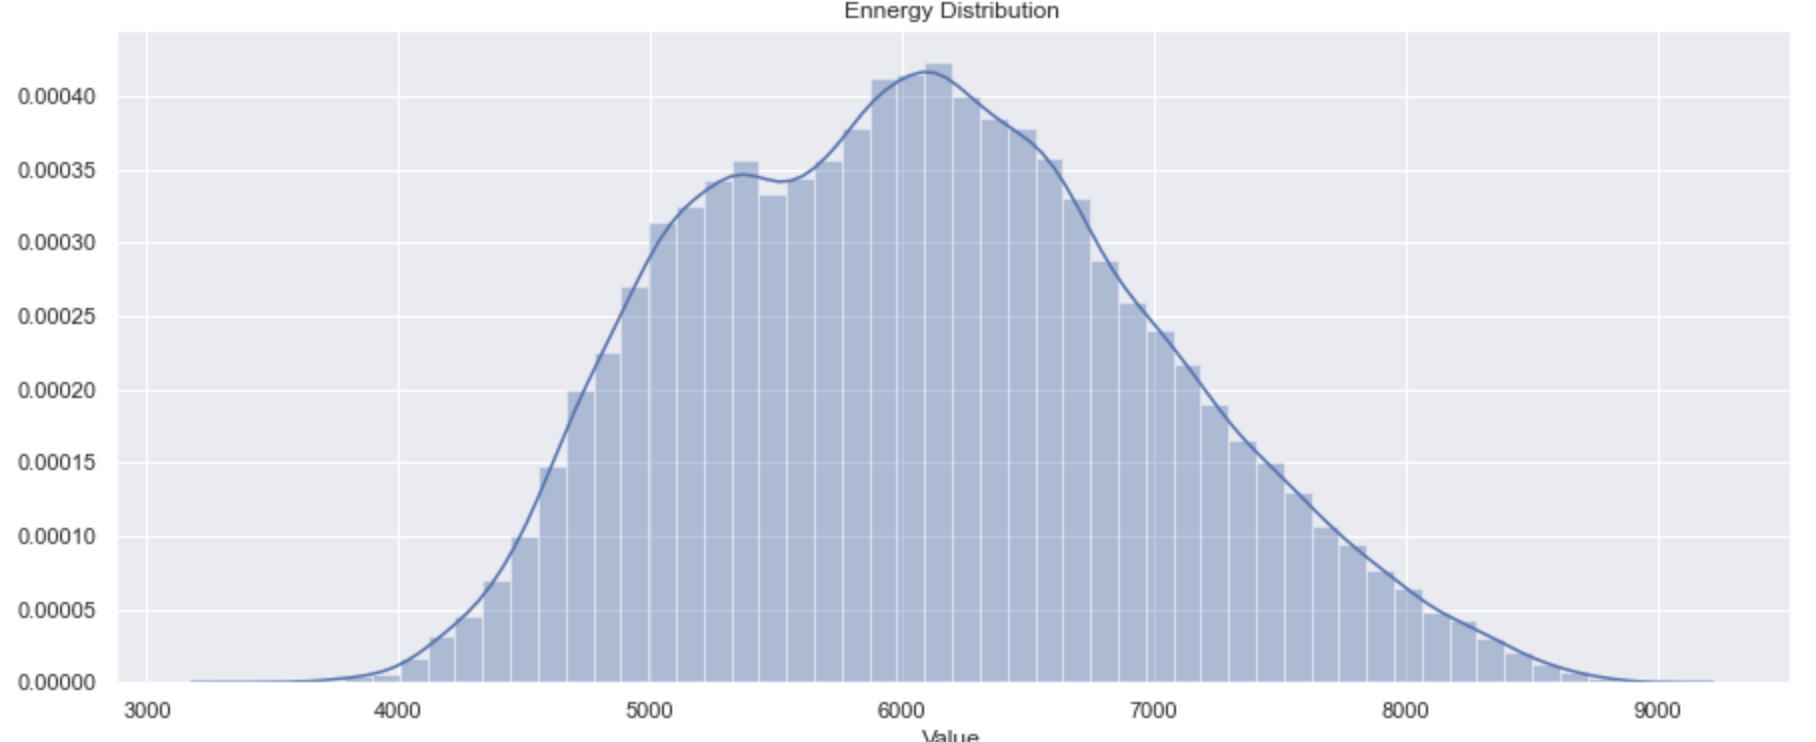
\includegraphics[width=\linewidth]{midterm-report-latex/energy.png}
\end{center}
   \caption{Distribution of energy consumption}
\end{figure}

\paragraph{Evaluation method:} 
The evaluation of the LSTM-model is done using a series of benchmark numbers, used in multiple studies that compare different options for EDF:
\begin{itemize}
\item Mean absolute error (MAE) and Root-mean-squared error (RMSE), which are absolute performance measures that allow us to compare the deviation between the actual values and the predictions.
\item MAPE, which is a relative measure that represents the forecasting error between the actual value and the prediction.
\end{itemize}

These indicators will be used both to evaluate the results of the LSTM model, as well as the results of the traditional ARIMA model. This will enable a robust comparative and allow us to deduce whether LSTM improves accuracy in predicting electricity consumption values based on historical data in the absence of weather-related information. This comprehensive evaluation of the model is one element of novelty that our project brings to the discussion. Usually, one indicator is chosen to compare and contrast a series of models. However, the choice appears to be random at best, and subjective at worst. In this sense, our agnostic positioning will allow us to properly deduce if from an accuracy perspective, the LSTM-based RNN model is superior to the non-ML ARIMA traditional model.

\paragraph{Experimental details:} 

First and foremost, the dataset has been separated into training and testing subsets. Because the intent of our project is to replicate the real-world tasks performed by network operators, splitting the dataset is not done through any algorithms, but by imposing a data-time threshold. Every hour before the threshold is thus part of the training set, while the hours after the threshold constitute the testing set. This method is in line with the literature in the field. 

Before the splitting, the model has been reshaped to display average values for each day (collections of 24 hour observations). This has been done for reasons of brevity, and we will experiment with different shapes in the upcoming weeks.This new data-set only contains 4991 observation, for each day between 01.01.2006 and 31.08.2019. While this is a significant reduction of the observations available for the model, there are two reasons for testing this re-sampling strategy: 
\begin{itemize}
\item Often times, EDF is used for determining the expected size of the balancing market, which is a daily market in the first place.
\item This allows us to see the accuracy of the model. Feeding more granular data is expected to improve how the LSTM behaves, so this acts as a good first experiment.
\end{itemize}

The results displayed in this mid-term report are based on a train-test split that uses only the last 75 time interval in the dataset for testing. While this might appear low, this follows industry practice, where years of data are used to predict electricity consumption for at most a couple of weeks, usually only for the day-ahead. 

\paragraph{Results:} 

\begin{figure}[H]
\begin{center}
   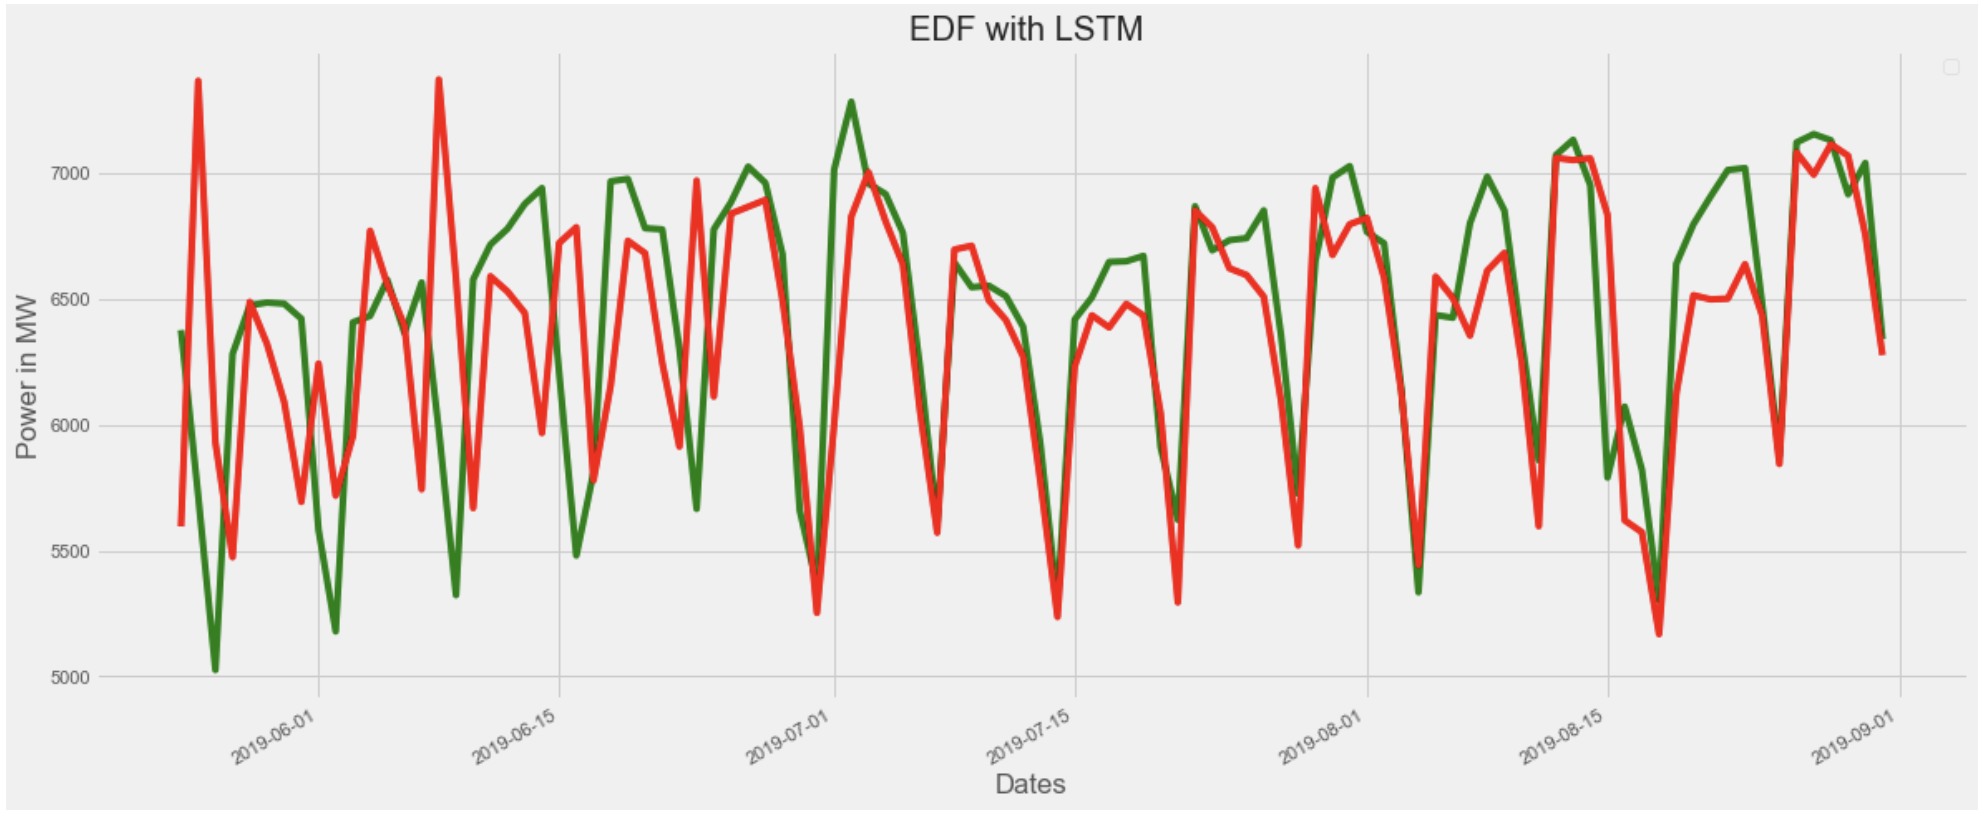
\includegraphics[width=\linewidth]{midterm-report-latex/LTSM_EDF.png}
\end{center}
   \caption{Re-sampled dataset}
\end{figure}

The figure below offers a sample of the results. The first visual evaluation hint towards the effectiveness of the model. This sample, as well as the plot in Figure 7, have been presented to the first human evaluator we had acquired for this project,the founder of a Romanian consultancy that offers EDF services for one of the largest electricity producers in the country, Hidroelectrica. There are two observations that we obtained: 
\begin{itemize}
\item Regarding the aggregate curve of the time series predicted, the model is impressively accurate given the conservative approach of not using weather data as additional inputs.
\item There is, however, a problem with the model overestimating the demand for electricity at some points. The LSTM predicts extreme spikes in the load consumed at some points during the year, which is inaccurate for the data in 2019. One explanation is the lack of energy efficiency measures in previous years, which can have drastic effects on the size of the load. 
\end{itemize}

A preliminary description of the baseline-ARIMA model can be seen below. This shows the limitations of econometric, non-ML models in the absence of weather-related data.


\begin{figure}[H]
\begin{center}
   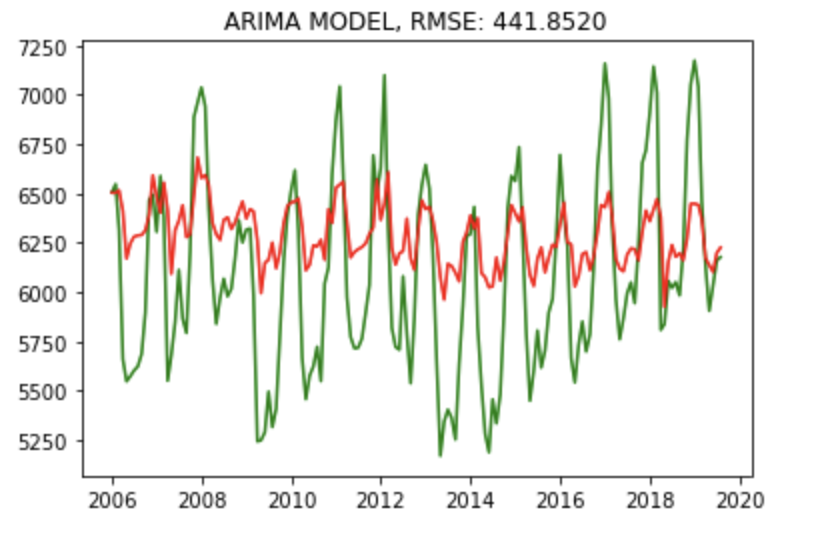
\includegraphics[width=\linewidth]{midterm-report-latex/ARIMA.png}
\end{center}
   \caption{Re-sampled dataset}
\end{figure}


\paragraph{Comment on your quantitative results.} The preliminary quantitative results show that our. LSTM-based RNN model has an accuracy similar to other models of this type that have been designed in the literature. Given that we only run a preliminary number of settings for the model, this is better than the originally expected results. 

One very important point is that our model accurately predicts the extreme points in the distributions, namely the spikes in electricity consumption, as well as the large drops. The following table displays the preliminary results of the model, based on the evaluation metrics previously described. 

\begin{center}
 \begin{tabular}{||c c c c||} 
 \hline
Evaluation metric & LSTM & ARIMA &\\ [0.5ex] 
 \hline\hline
 MAPE & 0.057 & TBD&\\ 
 \hline
 MAE & 350.66 & TBD &\\
 \hline
 RMSE & 519.76 & TBD & \\
 \hline
\end{tabular}
\end{center}

One intermediary conclusion is that without significant optimizations, the LSTM is able to offer accurate predictions even in the absence of information on weather for the historical data used as inputs. A proper comparison with the ARIMA and potentially with the RF will be provided.
\section{Future work}

\begin{itemize}
\item The first step will be to finish the implementation of the traditional ARIMA model. If everything runs smoothly, we will also see how shallow-ML model like a random forest performs in contrast to the deep-learning LSTM-based RNN and the ARIMA.
\item The second step is to create a database exploring how different model settings influence different types of models. These results will be evaluated both through the set of indicators described, and by a couple of human evaluators. Based on the dual-evaluation, we will provide a comprehensive qualitative analysis. 
\end{itemize}


\begin{thebibliography}{}

\bibitem  EEl-Mouden (2020)
\textit {Electricity consumption}.
https://github.com/drwiiche/electricity-consumption


\bibitem  HHochreiter and Schmidhuber (1997).
\textit {Long Short-Term Memory}.
Neural Computation, 9(8):1735-1780.

\bibitem LLago et al.(2018).
\textit{Forecasting spot electricity prices: Deep learning approaches and empirical comparison of traditional algorithms}. 
Applied Energy, 221:386-405.

\bibitem  MMuzaffar and Afshari (2019).
\textit{Short-Term Load Forecasts Using LSTM Networks}. 
Energy Procedia, 158:2922-2927.

\bibitem   SSon and Kim (2020)
\textit{Predicting Residential Energy Consumption using CNN-LSTM Neural Networks}. 
Energy, 182:72-81.

\bibitem    ZZheng  et  al (2017)
\textit{Electric load forecasting in smart grids using Long-Short-Term-Memory based Recurrent Neural Network}. 
51st Annual Conference on Information Sciences and Systems (CISS).





\end{thebibliography}



\end{document}
